\chapter{ANALISIS DAN PERANCANGAN SISTEM}
\par Bab ini membahas analisis dan perancangan sistem untuk mencapai tujuan dari tugas akhir, meliputi perancangan data, proses, dan analisa implementasi secara umum.

\section{Analisis Sistem}
\par Subbab ini membahas hasil analisa perangkat lunak push notification terpusat.
Analisis yang dilakukan meliputi analisis permasalahan, deskripsi umum sistem, dan spesifikasi kebutuhan perangkat lunak.

\subsection{Analisis Permasalahan}
\par Subbab ini membahas permasalahan yang dihadapi oleh Push Notification Terpusat saat ini, berupa penyebab, dampak, dan solusi dari masalah tersebut.

\subsubsection{Keandalan Antrian Pesan}
\par Proses pengolahan pesan yang ada di antrian saat ini dilakukan dengan membuat beberapa \textit{thread} yang bertindak sebagai \textit{producer} dan \textit{consumer} dari antrian pesan. \textit{Thread} tersebut akan menambahkan dan mengambil pesan dari antrian secara bersamaan.
\par Berdasarkan analisis yang penulis lakukan, struktur data \textit{linked list} yang digunakan oleh antrian tidak mendukung perubahan data secara bersamaan \cite{linkedlist-online}.
\par Konsekuensinya, bisa saja terjadi kasus \textit{race condition} yang menyebabkan pesan yang berada di antrian hilang tanpa ada \textit{error} yang terdeteksi oleh sistem. \textit{Race condition} adalah kondisi dimana beberapa proses mengakses sumber daya yang sama pada saat bersamaan, sehingga hasil akhir bergantung pada proses mana yang terakhir selesai dieksekusi. Potongan kode implementasi antrian pesan dapat dilihat pada \nameref{lampiran:queue_service}.
\par Salah satu solusi yang dapat digunakan untuk menyelesaikan masalah ini adalah dengan menggunakan Kafka sebagai perantara pesan. Arsitektur Kafka membagi antrian pesan berdasarkan topik dan partisi. Antrian pesan yang berada di satu topik dan partisi akan diolah secara \textit{synchronous}, dan jika berbeda topik atau partisi akan diolah secara \textit{asynchronous}. Arsitektur Kafka menjamin setiap antrian pesan hanya akan digunakan oleh satu \textit{producer} dan \textit{consumer} pada satu waktu, sehingga kasus \textit{race condition} dapat dihindarkan.

\subsubsection{Durabilitas Penyimpanan Antrian}
\par Proses penyimpanan pesan yang ada di antrian saat ini dilakukan dengan menyimpan pesan ke dalam sebuah struktur data \textit{linked list} yang ada di sistem.
\par Konsekuensinya, jika sistem mati, seluruh pesan yang berada diantrian akan hilang. Selain itu, karena semua pesan disimpan di sistem, sistem akan kehabisan memori dan \textit{crash} jika jumlah pesan yang diantrikan terlalu banyak.
\par Salah satu solusi yang dapat digunakan untuk menyelesaikan masalah ini adalah dengan menggunakan Kafka sebagai media penyimpanan antrian. Dengan memindahkan antrian pesan ke Kafka, maka antrian pesan tetap dapat berjalan meskipun sistem sedang mati. Kafka juga menyimpan data antrian pesan kedalam media penyimpanan server, sehingga meskipun Kafka mati, pesan tetap tersimpan dan dapat diolah kembali.

\subsection{Deskripsi Umum Sistem}
\par Push Notification Terpusat merupakan layanan yang digunakan untuk mengirim \textit{push notification} ke perangkat pengguna secara terjadwal dan \textit{asynchronous}. Alur pengiriman \textit{push notification} diawali dengan pengelola memasukkan data \textit{batch} (notifikasi yang dikirim ke beberapa pengguna atau kelompok pengguna) ke sistem basis data, lalu sistem akan mengolah data \textit{batch} menjadi \textit{packet-packet} (notifikasi yang dikirim ke satu perangkat pengguna). Setelah \textit{packet} dibuat, sistem akan mengirimkan \textit{packet} ke perangkat pengguna lewat layanan APNs dan FCM.
\par Pada tugas akhir ini, modul \textit{engine} pada Push Notification Terpusat akan dipecah menjadi 3 modul, yaitu Scheduler, Sender APN, dan Sender FCM. Secara umum, Scheduler bertanggung jawab untuk menjadwalkan dan mengantrikan \textit{packet}, Sender APN bertanggung jawab untuk mengirimkan \textit{packet} yang diantrikan ke perangkat iOS lewat layanan APNs, dan Sender FCM bertanggung jawab untuk mengirimkan \textit{packet} yang diantrikan ke perangkat Android dan Web lewat layanan FCM.

\subsection{Spesifikasi Kebutuhan Perangkat Lunak}
\par Subbab ini membahas spesifikasi kebutuhan perangkat lunak dari hasil analisis yang telah dilakukan. Subbab ini berisi kebutuhan perangkat lunak yang direpresentasikan dalam bentuk kebutuhan fungsional, kebutuhan non fungsional, dan diagram kasus penggunaan.

\subsubsection{Aktor}
\par Aktor adalah pihak-pihak, baik manusia maupun sistem atau perangkat lain yang terlibat dan berinteraksi secara langsung dengan sistem. Rincian aktor-aktor yang terdapat pada aplikasi push notification terpusat dijelaskan pada Tabel \ref{t:aktor}.
\begin{longtable}{|p{2cm}|p{7cm}|}
    \caption{Aktor pada Sistem} \label{t:aktor} \\ \hline
    \rowcolor{lightgray} Aktor & Tugas \\ \hline
    Manajemen & Membuat \textit{batch} dan melakukan pemantauan. \\ \hline
    Scheduler & Membuat dan menjadwalkan pengiriman \textit{packet}. \\ \hline
    Sender APN & Mengirimkan \textit{packet} untuk perangkat iOS. \\ \hline
    Sender FCM & Mengirimkan \textit{packet} notifikasi untuk perangkat Android dan Web. \\ \hline
\end{longtable}

\subsubsection{Kebutuhan Fungsional}
\par Kebutuhan fungsional mendefinisikan hal-hal yang harus dilakukan oleh sistem berdasarkan masukan yang diterima, proses yang dilakukan, dan hasil yang dicapai. Kebutuhan fungsional aplikasi push notification terpusat dijelaskan pada Tabel \ref{t:fungsional}.
\begin{longtable}{|p{1cm}|p{3cm}|p{5cm}|}
    \caption{Kebutuhan Fungsional Sistem} \label{t:fungsional} \\ \hline
    \rowcolor{lightgray} Kode & {Kebutuhan} & Deskripsi \\ \hline
    F-01 & Pembuatan \textit{Packet} & Jika terdapat \textit{batch} yang belum dan boleh dibuatkan \textit{packet}, sistem dapat membuatkan \textit{packet} dari \textit{batch} tersebut. \\ \hline
    F-02 & Menambahkan \textit{Packet} ke Antrian & Jika terdapat \textit{packet} yang belum dan sudah waktunya dikirim, sistem dapat menambahkan \textit{packet} tersebut ke antrian. \\ \hline
    F-03 & Pengiriman \textit{Packet} ke APNs & Jika terdapat \textit{packet} untuk perangkat iOS di antrian, sistem dapat mengambil \textit{packet} dari antrian dan mengirim \textit{packet} ke layanan APNs. \\ \hline
    F-04 & Pengiriman \textit{Packet} ke FCM & Jika terdapat \textit{packet} untuk perangkat Android dan Web di antrian, sistem dapat mengambil \textit{packet} dari antrian dan mengirim \textit{packet} ke layanan FCM. \\ \hline
    F05 & Menampilkan Penggunaan Sumber Daya & Jika mendapat \textit{request} HTTP tertentu, sistem dapat menampilkan penggunaan sumber daya (CPU dan Memori) yang digunakan dalam bentuk \textit{response} HTTP. \\ \hline
    F-06 & Menampilkan Status Kesehatan & Jika mendapat \textit{request} HTTP tertentu, sistem dapat menampilkan kondisi layanan yang berhubungan dengan sistem (sistem basis data dan antrian pesan) dalam bentuk \textit{response} HTTP. \\ \hline
    F-07 & Menampilkan Konfigurasi & Jika mendapat \textit{request} HTTP tertentu, sistem dapat menampilkan konfigurasi sistem dalam bentuk \textit{response} HTTP. \\ \hline
    F-08 & Menampilkan \textit{Log} & Jika mendapat \textit{request} HTTP tertentu, sistem dapat menampilkan isi \textit{log} sistem dalam bentuk \textit{response} HTTP. \\ \hline
\end{longtable}

\subsubsection{Kebutuhan Non Fungsional}
\par Kebutuhan non fungsional mendefinisikan bagaimana sistem harus bekerja dalam kondisi tertentu. Kebutuhan non fungsional aplikasi push notification terpusat dijelaskan pada Tabel \ref{t:non_fungsional}.
\begin{longtable}{|p{1.2cm}|p{2cm}|p{5.5cm}|}
	\caption{Kebutuhan Non Fungsional Sistem} \label{t:non_fungsional} \\ \hline
    \rowcolor{lightgray} Kode & Aspek & Deskripsi \\ \hline
    NF-01 & Performa & Aplikasi dapat mengirimkan 100 ribu \textit{push notification} dalam waktu kurang dari 6 jam. \\ \hline
    NF-02 & Keandalan & Aplikasi dapat mengirimkan 100 ribu \textit{push notification} ke layanan APNs dan FCM tanpa gagal. \\ \hline
    NF-03 & Ketersediaan & Aplikasi dapat menangani pengiriman 100 ribu \textit{push notification} tanpa ada layanan yang \textit{down}. \\ \hline
    NF-04 & Durabilitas & Aplikasi dapat mengirimkan \textit{push notification} saat salah satu layanan dimatikan sementara. \\ \hline
\end{longtable}

\subsubsection{Kasus Penggunaan}
\par Subbab ini membahas kasus penggunaan perangkat lunak secara rinci. Kasus penggunaan dibuat berdasarkan hasil analisis yang pada subbab sebelumnya. Diagram kasus penggunaan modul Scheduler, Sender APN, dan Sender FCM dapat dilihat pada Gambar \ref{img:uc-scheduler}, \ref{img:uc-sender_apn}, dan \ref{img:uc-sender_fcm}.
\begin{figure}[H]
    \centering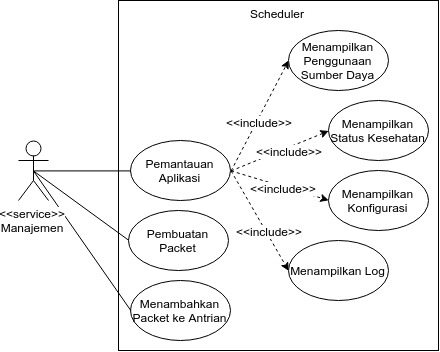
\includegraphics[width=0.7\textwidth]{bab3/img/usecase-scheduler.jpg}
    \caption{Diagram Kasus Penggunaan Scheduler} \label{img:uc-scheduler}
\end{figure}
\begin{figure}[H]
	\centering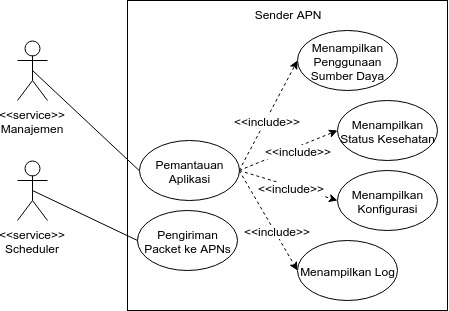
\includegraphics[width=0.7\textwidth]{bab3/img/usecase-sender_apn.jpg}
	\caption{Diagram Kasus Penggunaan Sender APN} \label{img:uc-sender_apn}
\end{figure}
\begin{figure}[H]
	\centering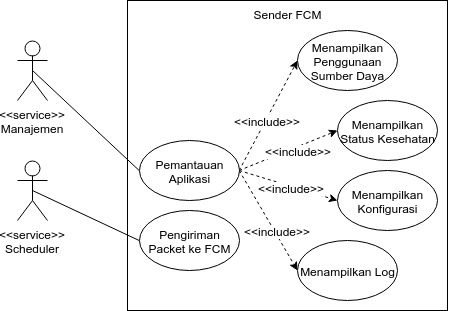
\includegraphics[width=0.7\textwidth]{bab3/img/usecase-sender_fcm.jpg}
	\caption{Diagram Kasus Penggunaan Sender FCM} \label{img:uc-sender_fcm}
\end{figure}

% template tabel deskripsi kasus penggunaan
\newcommand\tableUcDesc[8] {
\begin{longtable}{|p{2.5cm}|p{6.5cm}|}
	\caption{Kasus Penggunaan #3} \label{#1} \\ \hline
    \rowcolor{lightgray} Komponen & Deskripsi \\ \hline
    Kode & #2 \\ \hline
    Nama & #3 \\ \hline
    Aktor & #4 \\ \hline
    Kondisi Awal & #5 \\ \hline
    Kondisi Akhir & #6 \\ \hline
    Alur Normal & #7 \\ \hline
    Alur Alternatif & #8 \\ \hline
\end{longtable}
}

\clearpage

\paragraph{Pembuatan Packet}
\par Pada kasus ini, Scheduler akan mencari batch yang belum dan boleh dibuatkan \textit{packet} secara berkala. Jika ada, Scheduler akan membuatkan \textit{packet} untuk \textit{batch} tersebut. Rincian skenario dapat dilihat pada Tabel \ref{t:skenario_pembuatan_packet}.
\tableUcDesc
{t:skenario_pembuatan_packet}
{UC-01}
{Pembuatan \textit{Packet}}
{Manajemen}
{Terdapat \textit{batch} yang belum dan boleh dibuatkan \textit{packet}}
{\textit{Packet} dibuat untuk \textit{batch} tersebut}
{
\begin{enumerate}
	\item Aktor menambahkan data \textit{batch} baru ke sistem basis data.
    \item Scheduler mendeteksi data \textit{batch} yang belum dan boleh dibuatkan \textit{packet}.
    \item Scheduler membuatkan data \textit{packet} dari \textit{batch} tersebut.
    \item Scheduler menyimpan data \textit{packet} dan memperbarui data waktu pengolahan \textit{batch}.
\end{enumerate}
}
{-}
\clearpage

\paragraph{Menambahkan Packet ke Antrian}
\par Pada kasus ini, Scheduler akan mencari \textit{packet} yang belum dan sudah waktunya dikirim secara berkala. Jika ada, Scheduler akan menambahkan \textit{packet} tersebut ke antrian pesan dengan topik yang dibagi berdasarkan jenis perangkat penerima. Rincian skenario dapat dilihat pada Tabel \ref{t:skenario_menambahkan_packet_ke_antrian}.
\tableUcDesc
{t:skenario_menambahkan_packet_ke_antrian}
{UC-02}
{Menambahkan \textit{Packet} ke Antrian}
{Manajemen}
{Terdapat \textit{packet} yang belum dan sudah waktunya dikirim}
{\textit{Packet} ditambahkan ke antrian}
{
\begin{enumerate}
    \item Aktor menambahkan data \textit{batch} baru ke sistem basis data.
    \item Scheduler membuatkan \textit{packet} untuk \textit{batch} tersebut.
    \item Scheduler mendeteksi data \textit{packet} yang belum dan sudah waktunya dikirim.
    \item Scheduler memperbarui data status \textit{packet} menjadi menunggu untuk diolah.
    \item Scheduler menambahkan \textit{packet} ke antrian dengan menggunakan tipe perangkat sebagai topik.
\end{enumerate}
}
{-}
\clearpage

\paragraph{Pengiriman Packet ke APNs}
\par Pada kasus ini, Sender APN akan menunggu sistem antrian pesan untuk mengirimkan \textit{packet} yang ada di antrian topik iOS. Setelah packet diterima, packet akan dikirimkan ke layanan APNs. Rincian skenario dapat dilihat pada Tabel \ref{t:skenario_pengiriman_packet_ke_apns}.
\tableUcDesc
{t:skenario_pengiriman_packet_ke_apns}
{UC-03}
{Pengiriman \textit{Packet} ke APNs}
{Scheduler}
{Terdapat \textit{packet} di antrian topik iOS}
{\textit{Packet} diterima oleh layanan APNs}
{
\begin{enumerate}
	\item Aktor menambahkan \textit{packet} ke antrian topik iOS.
    \item Sender APN menerima \textit{packet} dari antrian topik iOS.
    \item Sender APN mengirimkan \textit{request push notification} ke layanan APNs berdasarkan data \textit{packet}.
    \item Sender APN memperbarui data \textit{packet} berdasarkan \textit{response} dari APNs (berhasil atau gagal dan alasan gagal).
\end{enumerate}
}
{-}
\clearpage

\paragraph{Pengiriman Packet ke FCM}
\par Pada kasus ini, Sender FCM akan menunggu sistem antrian pesan untuk mengirimkan \textit{packet} yang ada di antrian topik Android dan Web. Setelah \textit{packet} diterima, \textit{packet} akan dikirimkan ke layanan FCM. Rincian skenario dapat dilihat pada Tabel \ref{t:skenario_pengiriman_packet_ke_fcm}.
\tableUcDesc
{t:skenario_pengiriman_packet_ke_fcm}
{UC-04}
{Pengiriman \textit{Packet} ke FCM}
{Scheduler}
{Terdapat \textit{packet} di antrian topik Android atau Web}
{Packet diterima oleh layanan FCM}
{
\begin{enumerate}
	\item Aktor menambahkan \textit{packet} ke antrian topik Android atau Web.
    \item Sender FCM menerima packet dari antrian topik Android atau Web.
    \item Sender FCM mengirimkan \textit{request push notification} ke layanan FCM berdasarkan data \textit{packet}.
    \item Sender FCM memperbarui data \textit{packet} berdasarkan \textit{response} dari FCM (berhasil atau gagal dan alasan gagal).
\end{enumerate}
}
{-}
\clearpage

\paragraph{Menampilkan Penggunaan Sumber Daya}
\par Pada kasus ini, Scheduler, Sender APN, dan Sender FCM dapat menampilkan penggunaan sumber daya (CPU dan Memori) yang digunakan aplikasi. Rincian skenario dapat dilihat pada Tabel \ref{t:skenario_menampilkan_penggunaan_sumber_daya}.
\tableUcDesc
{t:skenario_menampilkan_penggunaan_sumber_daya}
{UC-05}
{Menampilkan Penggunaan Sumber Daya}
{Manajemen}
{Aktor mengirimkan \textit{request} HTTP untuk melihat penggunaan sumber daya}
{Sistem mengembalikan \textit{response} HTTP}
{
\begin{enumerate}
	\item Aktor mengirimkan \textit{request} HTTP untuk melihat penggunaan sumber daya.
	\item Scheduler, Sender APN, atau Sender FCM memeriksa metrik penggunaan sumber daya dari sistem operasi.
	\item Scheduler, Sender APN, atau Sender FCM mengembalikan hasil pemeriksaan penggunaan sumber daya dalam bentuk \textit{response} HTTP.
\end{enumerate}
}
{-}
\clearpage

\paragraph{Menampilkan Status Kesehatan}
\par Pada kasus ini, Scheduler, Sender APN, dan Sender FCM dapat menampilkan status kesehatan aplikasi dan layanan yang terhubung dengan aplikasi. Rincian skenario dapat dilihat pada Tabel \ref{t:skenario_menampilkan_status_kesehatan}.
\tableUcDesc
{t:skenario_menampilkan_status_kesehatan}
{UC-06}
{Menampilkan Status Kesehatan}
{Manajemen}
{Manajemen mengirimkan \textit{request} HTTP untuk melihat status kesehatan}
{Sistem mengembalikan \textit{response} HTTP}
{
\begin{enumerate}
	\item Aktor mengirimkan \textit{request} HTTP untuk melihat status kesehatan.
	\item Scheduler, Sender APN, atau Sender FCM memeriksa apakah aktor dapat terhubung ke layanan-layanan yang dibutuhkan oleh aktor untuk beroperasi.
	\item Scheduler, Sender APN, atau Sender FCM mengembalikan status (bisa diakses atau tidak) layanan-layanan yang dibutuhkan dalam bentuk \textit{response} HTTP.
\end{enumerate}
}
{-}
\clearpage

\paragraph{Menampilkan Konfigurasi}
\par Pada kasus ini, Scheduler, Sender APN, dan Sender FCM dapat menampilkan konfigurasi aplikasi. Rincian skenario dapat dilihat pada Tabel \ref{t:skenario_menampilkan_konfigurasi}.
\tableUcDesc
{t:skenario_menampilkan_konfigurasi}
{UC-07}
{Menampilkan Konfigurasi}
{Manajemen}
{Aktor mengirimkan \textit{request} HTTP untuk melihat konfigurasi}
{Sistem mengembalikan \textit{response} HTTP}
{
	\begin{enumerate}
		\item Aktor mengirimkan \textit{request} HTTP untuk melihat konfigurasi aplikasi.
		\item Scheduler, Sender APN, atau Sender FCM memeriksa konfigurasi \textit{Spring} yang digunakan.
		\item Scheduler, Sender APN, atau Sender FCM memeriksa \textit{environment variable} yang ada di sistem operasi.
		\item Scheduler, Sender APN, atau Sender FCM mengembalikan konfigurasi \textit{Spring} dan \textit{environment variable} yang ada dalam bentuk \textit{response} HTTP.
	\end{enumerate}
}
{-}
\clearpage

\paragraph{Menampilkan Log}
\par Pada kasus ini, Scheduler, Sender APN, dan Sender FCM dapat menampilkan \textit{log} yang dikeluarkan oleh aplikasi dengan menggunakan REST API. Rincian skenario dapat dilihat pada Tabel \ref{t:skenario_menampilkan_log}.
\tableUcDesc
{t:skenario_menampilkan_log}
{UC-08}
{Menampilkan \textit{Log}}
{Manajemen}
{Aktor mengirimkan \textit{request} HTTP untuk melihat \textit{log}}
{Sistem mengembalikan \textit{response} HTTP}
{
\begin{enumerate}
	\item Aktor mengirimkan \textit{request} HTTP untuk melihat log aplikasi.
	\item Scheduler, Sender APN, atau Sender FCM mencari lokasi file \textit{log} yang digunakan untuk menyimpan \textit{log}.
	\item Scheduler, Sender APN, atau Sender FCM mengembalikan isi file \textit{log} dalam bentuk \textit{response} HTTP.
\end{enumerate}
}
{-}
\clearpage

\section{Perancangan Sistem}
\par Subbab ini akan membahas tahapan perancangan sistem yang dibagi menjadi beberapa bagian, yaitu perancangan arsitektur, basis data, antrian pesan, dan proses.

\subsection{Perancangan Arsitektur} \label{s:perancangan_arsitektur}
\par Modul engine pada Push Notification Terpusat akan dibagi menjadi 3 modul, yaitu Scheduler, Sender APN, dan Sender FCM. Modul Push Notification Terpusat diimplementasikan dengan bahasa pemrograman Java, dengan kerangka kerja Spring. Aplikasi saling terhubung lewat sistem antrian pesan (Kafka) dan sistem basis data (SQL Server).
\par Untuk menjalankan sistem, modul Push Notification Terpusat, Kafka, dan Zookeeper akan dijalankan menggunakan Docker, dan SQL Server menggunakan server basis data ITS. Secara garis besar, aplikasi ini memiliki rancangan arsitektur yang dapat dilihat pada Gambar \ref{img:arsitektur_baru}.
\begin{figure}[H]
    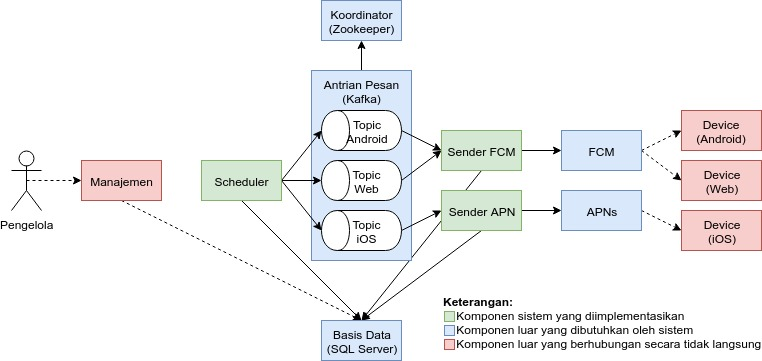
\includegraphics[width=1\textwidth]{bab3/img/arsitektur-push_notification_terpusat_baru.jpg}
    \caption{Rancangan Arsitektur Push Notification Terpusat} \label{img:arsitektur_baru}
\end{figure}

\subsection{Perancangan Basis Data}
\par Subbab ini membahas bagaimana rancangan basis data yang digunakan pada aplikasi \textit{push notification} terpusat. Sistem basis data yang digunakan adalah SQL Server. \textit{Conceptual Data Model} dan \textit{Physical Data Model} dapat dilihat pada \nameref{lampiran:cdm} dan \nameref{lampiran:pdm}.

\subsubsection{Tabel User}
\par Tabel User digunakan untuk menyimpan data pengguna aplikasi yang ada di Institut Teknologi Sepuluh Nopember. Rincian atribut dapat dilihat pada Tabel \ref{tabel_user}.
\begin{longtable}{|p{2cm}|p{2.5cm}|p{4.5cm}|}
 	\caption{Tabel User} \label{tabel_user} \\ \hline
    \rowcolor{lightgray} {Atribut} & {Tipe Data} & {Deskripsi} \\ \hline
    User ID & uuid & ID tabel \\ \hline
    Name & varchar(150) & Nama dari akun ITS \\ \hline
%    Nickname & varchar(20) & - \\ \hline
%    Username & varchar(255) & - \\ \hline
%    Password & varchar(256) & - \\ \hline
    Email & varchar(255) & NRP/NIP/no telepon dari akun ITS \\ \hline
%    Email Verified & numeric(1) & - \\ \hline
%    Scope & varchar(4000) & - \\ \hline
%    Alternate Email & varchar(255) & - \\ \hline
%    Alternate Email Verified & numeric(1) & - \\ \hline
%    Phone & varchar(18) & - \\ \hline
%    Phone Verified & numeric(1) & - \\ \hline
%    Enabled & numeric(1) & - \\ \hline
%    Picture & varbinary(max) & - \\ \hline
%    Gender & char(1) & - \\ \hline
%    Birth Date & date & - \\ \hline
%    Zone Info & varchar(40) & - \\ \hline
%    Locale & varchar(10) & - \\ \hline
%    Integra ID & numeric(12) & - \\ \hline
%    Registration ID & varchar(25) & - \\ \hline
%    Must Change Password & numeric(1) & - \\ \hline
%    Sandbox & numeric(1) & - \\ \hline
%    Locked & datetime & - \\ \hline
%    Suspended & datetime & - \\ \hline
%    Has Suspended & numeric(1) & - \\ \hline
%    Group ID & int & - \\ \hline
%    Auth Method ID & numeric(2) & - \\ \hline
    Created At & datetime & Tanggal dan waktu dibuat \\ \hline
    Update At & datetime & Tanggal dan waktu diperbarui \\ \hline
\end{longtable}

\subsubsection{Tabel Group}
\par Tabel group digunakan untuk menyimpan data kelompok pengguna. Rincian atribut dapat dilihat pada Tabel \ref{tabel_group}.
\begin{longtable}{|p{2cm}|p{2.5cm}|p{4.5cm}|}
	\caption{Tabel Group} \label{tabel_group} \\ \hline
    \rowcolor{lightgray} {Atribut} & {Tipe Data} & {Deskripsi} \\ \hline
    Group ID & uuid & ID tabel \\ \hline
    Name & varchar(100) & Nama kelompok \\ \hline
    Created At & datetime & Tanggal dan waktu dibuat \\ \hline
    Update At & datetime & Tanggal dan waktu diperbarui \\ \hline
\end{longtable}

\subsubsection{Tabel Group Member}
\par Tabel group member digunakan untuk menyimpan data pengguna yang menjadi anggota dari suatu kelompok. Rincian atribut dapat dilihat pada Tabel \ref{tabel_group_member}.
\begin{longtable}{|p{2cm}|p{2.5cm}|p{4.5cm}|}
	\caption{Tabel Group Member} \label{tabel_group_member} \\ \hline
    \rowcolor{lightgray} {Atribut} & {Tipe Data} & {Deskripsi} \\ \hline
    Group ID & uuid & Grup tempat pengguna terdaftar \\ \hline
    User ID & uuid & Pengguna yang terdaftar di grup \\ \hline
    Created At & datetime & Tanggal dan waktu dibuat \\ \hline
    Update At & datetime & Tanggal dan waktu diperbarui \\ \hline
\end{longtable}

\subsubsection{Tabel Client}
\par Tabel client digunakan untuk menyimpan data aplikasi yang ada di Institut Teknologi Sepuluh Nopember. Rincian atribut dapat dilihat pada Tabel \ref{tabel_client}.
\begin{longtable}{|p{2cm}|p{2.5cm}|p{4.5cm}|}
	\caption{Tabel Client} \label{tabel_client} \\ \hline
    \rowcolor{lightgray} {Atribut} & {Tipe Data} & {Deskripsi} \\ \hline
    Client ID & uuid & ID tabel \\ \hline
    Client Name & varchar(100) & Nama aplikasi ITS \\ \hline
%    Client Description & varchar(250) & - \\ \hline
%    Client Secret & varchar(255) & - \\ \hline
%    Expires At & datetime & - \\ \hline
%    Logo & varchar(100) & - \\ \hline
%    Redirect URI & varchar(2000) & - \\ \hline
%    Post Logout Redirect URIS & varchar(2048) & - \\ \hline
%    Front Channel Logout URI & varchar(255) & - \\ \hline
%    Front Channel Logout Session Required & numeric(1) & - \\ \hline
%    Back Channel Logout URI & varchar(255) & - \\ \hline
%    Back Channel Logout Session Required & numeric(1) & - \\ \hline
%    Base URI & varchar(255) & - \\ \hline
%    API Base URI & varchar(255) & - \\ \hline
%    Application Type & char(1) & - \\ \hline
%    Contact Name & varchar(255) & - \\ \hline
%    Contact Email & varchar(255) & - \\ \hline
%    Preauthorized & numeric(1) & - \\ \hline
%    Grant Types & varchar(80) & - \\ \hline
%    Scope & varchar(4000) & - \\ \hline
%    Sandbox & numeric(1) & - \\ \hline
    Is Moderated & numeric(1) & Status moderasi dari aplikasi ITS (1/0) \\ \hline
%    Visible & numeric(1) & - \\ \hline
%    Category ID & int & - \\ \hline
%    Auth Type ID & char(1) & - \\ \hline
%    User ID & uuid & - \\ \hline
%    Provider ID & uuid & - \\ \hline
    Created At & datetime & Tanggal dan waktu dibuat \\ \hline
    Update At & datetime & Tanggal dan waktu diperbarui \\ \hline
\end{longtable}

\subsubsection{Tabel Certificate}
\par Tabel Certificate digunakan untuk menyimpan data sertifikat yang digunakan untuk autentikasi ke layanan APNs dan FCM. Rincian atribut dapat dilihat pada Tabel \ref{tabel_certificate}.
\begin{longtable}{|p{2cm}|p{2.5cm}|p{4.5cm}|}
	\caption{Tabel Certificate} \label{tabel_certificate} \\ \hline
    \rowcolor{lightgray} {Atribut} & {Tipe Data} & {Deskripsi} \\ \hline
    Certificate ID & uuid & ID tabel \\ \hline
    Client ID & uuid & ID Aplikasi yang menggunakan sertifikat \\ \hline
    Bundle ID & varchar(255) & Bundle ID untuk aplikasi iOS \\ \hline
    Certificate Key & text & File sertifikat yang sudah diencode dengan base64 \\ \hline
    Type & char(1) & Tipe sertifikat (FCM(1) atau APNs(2)) \\ \hline
    Password & varchar(255) & Kata sandi untuk sertifikat iOS \\ \hline
\end{longtable}

\subsubsection{Tabel Device}
\par Tabel Device digunakan untuk menyimpan data perangkat pengguna aplikasi yang terdaftar di layanan APNs dan FCM. Rincian atribut dapat dilihat pada Tabel \ref{tabel_device}.
\begin{longtable}{|p{2cm}|p{2.5cm}|p{4.5cm}|}
	\caption{Tabel Device} \label{tabel_device} \\ \hline
    \rowcolor{lightgray} {Atribut} & {Tipe Data} & {Deskripsi} \\ \hline
    Device ID & uuid & ID tabel \\ \hline
    Client ID & uuid & ID aplikasi tempat perangkat terdaftar \\ \hline
    User ID & uuid & ID pengguna pemilik perangkat \\ \hline
    Device Token & varchar(255) & Token yang terdaftar di layanan APNs dan FCM \\ \hline
    Device Type & char(1) & Jenis perangkat (Android(A), Web(W), atau iOS(I)) \\ \hline
    Active & numeric(1) & Perangkat aktif atau tidak \\ \hline
    Registration Date & datetime & Waktu dan tanggal perangkat didaftarkan \\ \hline
    Invalidate Date & datetime & Waktu dan tanggal perangkat dihapus \\ \hline
\end{longtable}

\subsubsection{Tabel Batch}
\par Tabel Batch digunakan untuk menyimpan data notifikasi yang akan dikirim ke beberapa pengguna atau kelompok pengguna. Rincian atribut dapat dilihat pada Tabel \ref{tabel_batch}.
\begin{longtable}{|p{2cm}|p{2.5cm}|p{4.5cm}|}
	\caption{Tabel Batch} \label{tabel_batch} \\ \hline
    \rowcolor{lightgray} {Atribut} & {Tipe Data} & {Deskripsi} \\ \hline
    Batch ID & uuid & ID tabel \\ \hline
    Title & varchar(255) & Judul notifikasi \\ \hline
    Body & varchar(255) & Isi pesan notifikasi \\ \hline
    Image & varchar(255) & Nama atau URL Gambar \\ \hline
    Sound & varchar(255) & Nama atau URL Suara \\ \hline
    Action & varchar(255) & Nama aksi yang dijalankan jika notifikasi dibuka \\ \hline
    Additional Data & varchar(255) & Data tambahan dengan format JSON \\ \hline
    Delivery Date & datetime & Waktu notifikasi dikirim \\ \hline
    Started Date & datetime & Waktu \textit{batch} mulai diproses \\ \hline
    Finished Date & datetime & Waktu \textit{batch} selesai diproses \\ \hline
    Is Allowed & numeric(1) & \textit{Batch} boleh diproses atau tidak \\ \hline
    User Sender ID & uuid & ID pengguna pembuat \textit{batch} \\ \hline
    Client Sender ID & uuid & ID aplikasi pembuat \textit{batch} \\ \hline
    Client Destination ID & uuid & ID aplikasi penerima notifikasi \\ \hline
    Created At & datetime & Tanggal dan waktu dibuat \\ \hline
    Update At & datetime & Tanggal dan waktu diperbarui \\ \hline
\end{longtable}

\subsubsection{Tabel User Destination}
\par Tabel User Destination digunakan untuk menyimpan data pengguna yang menjadi target penerima notifikasi dalam satu \textit{batch}. Rincian atribut dapat dilihat pada Tabel \ref{tabel_user_destination}.
\begin{longtable}{|p{2cm}|p{2.5cm}|p{4.5cm}|}
	\caption{Tabel User Destination} \label{tabel_user_destination} \\ \hline
    \rowcolor{lightgray} {Atribut} & {Tipe Data} & {Deskripsi} \\ \hline
    Batch ID & uuid & ID \textit{batch} yang dituju \\ \hline
    User ID & uuid & ID pengguna penerima notifikasi \\ \hline
    Created At & datetime & Tanggal dan waktu dibuat \\ \hline
    Update At & datetime & Tanggal dan waktu diperbarui \\ \hline
\end{longtable}

\subsubsection{Tabel Group Destination}
\par Tabel Group Destination digunakan untuk menyimpan data kelompok yang menjadi target penerima notifikasi dalam satu \textit{batch}. Rincian atribut dapat dilihat pada Tabel \ref{tabel_group_destination}.
\begin{longtable}{|p{2cm}|p{2.5cm}|p{4.5cm}|}
	\caption{Tabel Group Destination} \label{tabel_group_destination} \\ \hline
    \rowcolor{lightgray} {Atribut} & {Tipe Data} & {Deskripsi} \\ \hline
    Batch ID & uuid & ID \textit{batch} yang dituju \\ \hline
    Group ID & uuid & ID kelompok penerima notifikasi \\ \hline
    Created At & datetime & Tanggal dan waktu dibuat \\ \hline
    Update At & datetime & Tanggal dan waktu diperbarui \\ \hline
\end{longtable}

\subsubsection{Tabel Packet} \label{s:tabel_packet}
\par Tabel Packet digunakan untuk menyimpan data notifikasi yang dikirim ke satu perangkat. Rincian atribut dapat dilihat pada Tabel \ref{tabel_packet}.
\begin{longtable}{|p{2cm}|p{2.5cm}|p{4.5cm}|}
	\caption{Tabel Packet} \label{tabel_packet} \\ \hline
	\rowcolor{lightgray} {Atribut} & {Tipe Data} & {Deskripsi} \\ \hline
	Packet ID & uuid & ID tabel \\ \hline
	Batch ID & uuid & ID \textit{batch} yang digunakan \\ \hline
	Device Token ID & uuid & ID perangkat penerima notifikasi \\ \hline
	Sent At & datetime & Waktu notifikasi diterima oleh APNs atau FCM \\ \hline
	Reason & varchar(255) & Penyebab jika terjadi kegagalan \\ \hline
	Packet Status & numeric(1) & Status pengiriman packet (dibuat(1), menunggu(2), berhasil(3), atau gagal(4)) \\ \hline
	Created At & datetime & Tanggal dan waktu dibuat \\ \hline
	Update At & datetime & Tanggal dan waktu diperbarui \\ \hline
\end{longtable}

\subsection{Perancangan Antrian Pesan}
\par Subbab ini membahas bagaimana rancangan antrian pesan yang akan digunakan. Sistem antrian pesan yang digunakan adalah Kafka.

\subsubsection{Perancangan Skema}
\par Berdasarkan rancangan arsitektur pada Subbab \ref{s:perancangan_arsitektur}, Scheduler akan mengirimkan \textit{packet} ke Sender APN dan Sender FCM lewat antrian pesan. Pertukaran data \textit{packet} di antrian pesan akan menggunakan format JSON. Skema JSON dapat dilihat pada Kode Sumber \ref{json:packet}.
\lstinputlisting[label=json:packet, caption=Skema JSON \textit{Packet}, language=SQL] {bab3/json/packet.json}

\subsubsection{Perancangan Topik}
\par Berdasarkan rancangan arsitektur pada Subbab \ref{s:perancangan_arsitektur}, antrian \textit{packet} akan dipisah berdasarkan tipe perangkat penerima \textit{packet}. Rincian pembagian topik dapat dilihat pada Tabel \ref{t:pembagian_topik_antrian}.
\begin{longtable}{|p{2cm}|p{2cm}|p{5cm}|}
	\caption{Pembagian Topik Antrian} \label{t:pembagian_topik_antrian} \\ \hline
	\rowcolor{lightgray} Perangkat & Topik & Deskripsi \\ \hline
	Android & android & Berisi \textit{packet} untuk perangkat Android. \\ \hline
	Web & web & Berisi \textit{packet} untuk perangkat Web. \\ \hline
	iOS & ios & Berisi \textit{packet} untuk perangkat iOS. \\ \hline
\end{longtable}

\subsection{Perancangan Proses}
\par Subbab ini menjelaskan tentang rancangan, tujuan, dan diagram alir proses-proses yang ada pada aplikasi \textit{push notification} terpusat.

\subsubsection{Proses Pembuatan Packet}
\par Proses ini bertujuan untuk membuat \textit{packet} dari \textit{batch} yang baru dibuat. Proses pembuatan dapat dilihat di diagram alir pada Gambar \ref{flowchart_pembuatan_packet}.
\begin{figure}[H]
	\centering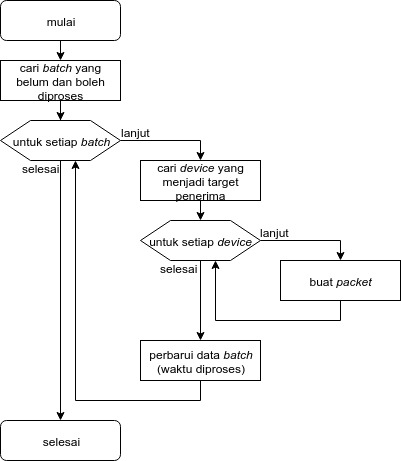
\includegraphics[width=0.8\textwidth]{bab3/img/flowchart-pembuatan_packet.jpg}
	\caption{Diagram Alir Proses Pembuatan Packet} \label{flowchart_pembuatan_packet}
\end{figure}
\clearpage

\subsubsection{Proses Menambahkan Packet ke Antrian}
\label{3:proses_menambahkan_packet_ke_antrian}
\par Proses ini bertujuan untuk mengantrikan \textit{packet} yang sudah waktunya untuk dikirim.
Antrian \textit{packet} dibagi berdasarkan jenis perangkat penerima notifikasi (Android, Web, atau iOS). Proses pengantrian dapat dilihat di diagram alir pada Gambar \ref{flowchart_menambahkan_packet_ke_antrian}.
\begin{figure}[H]
    \centering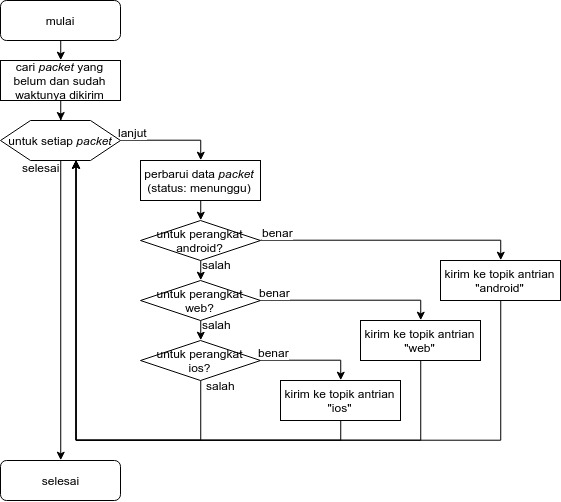
\includegraphics[width=1\textwidth]{bab3/img/flowchart-menambahkan_packet_ke_antrian.jpg}
    \caption{Diagram Alir Proses Menambahkan Packet ke Antrian} \label{flowchart_menambahkan_packet_ke_antrian}
\end{figure}
\clearpage

\subsubsection{Proses Pengiriman Packet ke APNs}
\par Proses ini bertujuan untuk mengirimkan \textit{packet} yang ada di antrian topik "ios" ke perangkat pengguna yang berbasis iOS lewat layanan APNs. Proses pengiriman \textit{packet} dapat dilihat di diagram alir pada
Gambar \ref{flowchart_pengiriman_packet_ke_apns}.
\begin{figure}[H]
    \centering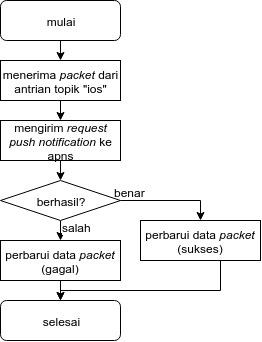
\includegraphics[width=0.6\textwidth]{bab3/img/flowchart-pengiriman_packet_ke_apns.jpg}
    \caption{Diagram Alir Proses Pengiriman Packet ke APNs} \label{flowchart_pengiriman_packet_ke_apns}
\end{figure}
\clearpage

\subsubsection{Proses Pengiriman Packet ke FCM}
\par Proses ini bertujuan untuk mengirimkan \textit{packet} yang ada di antrian topik "android" dan "web" ke perangkat pengguna yang berbasis Android atau Web lewat layanan FCM. Proses pengiriman \textit{packet} dapat dilihat di diagram alir pada Gambar \ref{flowchart_pengiriman_packet_ke_fcm}.
\begin{figure}[H]
    \centering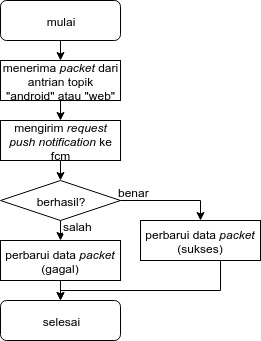
\includegraphics[width=0.6\textwidth]{bab3/img/flowchart-pengiriman_packet_ke_fcm.jpg}
    \caption{Diagram Alir Proses Pengiriman Packet ke FCM} \label{flowchart_pengiriman_packet_ke_fcm}
\end{figure}
\clearpage

\subsubsection{Proses Menampilkan Penggunaan Sumber Daya}
\par Proses ini bertujuan untuk menampilkan penggunaan sumber daya (seperti CPU dan Memori) yang digunakan oleh aplikasi. Proses menampilkan penggunaan sumber daya dapat dilihat di diagram alir pada Gambar \ref{fc:sumber_daya}.
\begin{figure}[H]
	\centering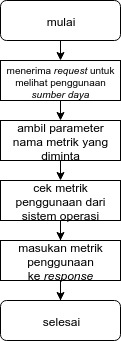
\includegraphics[width=0.4\textwidth]{bab3/img/flowchart-menampilkan_penggunaan_sumber_daya.jpg}
	\caption{Diagram Alir Proses Menampilkan Penggunaan Sumber Daya} \label{fc:sumber_daya}
\end{figure}
\clearpage

\subsubsection{Proses Menampilkan Status Kesehatan}
\par Proses ini bertujuan untuk menampilkan status kesehatan aplikasi dengan layanan-layanan yang dibutuhkan oleh aplikasi, yaitu sistem basis data dan sistem antrian pesan. Proses menampilkan status kesehatan dapat di diagram alir pada Gambar \ref{fc:kesehatan}.
\begin{figure}[H]
	\centering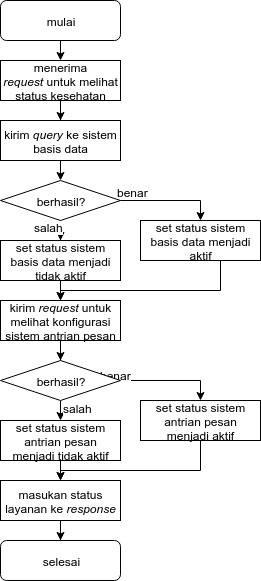
\includegraphics[width=0.5\textwidth]{bab3/img/flowchart-menampilkan_kesehatan.jpg}
	\caption{Diagram Alir Proses Menampilkan Status Kesehatan} \label{fc:kesehatan}
\end{figure}
\clearpage

\subsubsection{Proses Menampilkan Konfigurasi}
\par Proses ini bertujuan untuk menampilkan konfigurasi aplikasi dan lingkungan aplikasi yang digunakan untuk menjalankan aplikasi. Proses menampilkan konfigurasi dapat dilihat di diagram alir pada Gambar \ref{fc:konfigurasi}.
\begin{figure}[H]
	\centering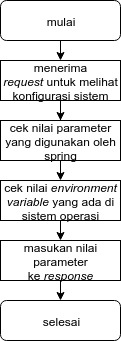
\includegraphics[width=0.4\textwidth]{bab3/img/flowchart-menampilkan_konfigurasi.jpg}
	\caption{Diagram Alir Proses Menampilkan Konfigurasi} \label{fc:konfigurasi}
\end{figure}
\clearpage

\subsubsection{Menampilkan Log}
\par Proses ini bertujuan untuk menampilkan \textit{log} yang dikeluarkan oleh aplikasi. Proses menampilkan \textit{log} dapat dilihat di diagram alir pada Gambar \ref{fc:log}.
\begin{figure}[H]
	\centering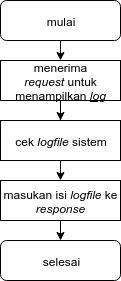
\includegraphics[width=0.4\textwidth]{bab3/img/flowchart-menampilkan_log.jpg}
	\caption{Diagram Alir Proses Menampilkan Log} \label{fc:log}
\end{figure}
\clearpage

\subsection{Perancangan API Endpoint}
\par Pemantauan Scheduler, Sender APN, dan Sender FCM menggunakan pustaka Actuator. Rincian API Endpoint yang digunakan untuk melihat hasil pemantauan dapat dilihat pada Tabel \ref{t:rancangan_api}.
\begin{longtable}[H]{|p{0.5cm}|p{3.5cm}|p{1.2cm}|p{3.5cm}|}
	\caption{Perancangan API Endpoint} \label{t:rancangan_api} \\ \hline
	\rowcolor{lightgray} No & Endpoint URI & Method & Deskripsi \\ \hline
	1 & /actuator/metrics/\newline process.uptime & GET & Menampilkan lama waktu sistem berjalan \\ \hline
	2 & /actuator/metrics/\newline process.cpu.usage & GET & Menampilkan penggunaan CPU oleh JVM \\ \hline
	3 & /actuator/metrics/\newline system.cpu.usage & GET & Menampilkan penggunaan CPU oleh sistem \\ \hline
	4 & /actuator/metrics/\newline system.cpu.count & GET & Menampilkan jumlah \textit{processor} yang bisa digunakan JVM \\ \hline
	5 & /actuator/metrics/\newline jvm.memory.used & GET & Menampilkan jumlah memori yang sedang digunakan \\ \hline
	6 & /actuator/metrics/\newline jvm.memory.max & GET & Menampilkan jumlah memori maksimum yang bisa digunakan \\ \hline
	7 & /actuator/metrics/\newline jvm.memory.committed & GET & Menampilkan jumlah memori yang digunakan oleh JVM \\ \hline
	8 & /actuator/health & GET & Menampilkan status kondisi kesehatan sistem basis data dan antrian pesan \\ \hline
	9 & /actuator/env & GET & Menampilkan konfigurasi sistem \\ \hline
	10 & /actuator/logfile & GET & Menampilkan isi \textit{log} \\ \hline
\end{longtable}
